\documentclass[12pt,unknownkeysallowed]{beamer}
\usetheme{Warsaw}
\setbeamertemplate{navigation symbols}{}
\mode<presentation>

\usepackage[utf8]{inputenc}
\usepackage[francais]{babel}
\usepackage[T1]{fontenc}
\usepackage[footheight=1em]{beamerthemeboxes}
\usepackage{graphicx}
\usepackage{color,listings}

\title{Présentation mi-projet}

\subtitle{Robot télécommandé par téléphone}

\author{Hugo GYBELS \and Claude-Alban RANÉLY}


\date{\today}

\addtobeamertemplate{navigation symbols}{}{%
		\usebeamerfont{footline}%
		\usebeamercolor[fg]{footline}%
		\hspace{1em}%
		\insertframenumber/\inserttotalframenumber
	}

\lstdefinestyle{Arduino}{%
    style=FormattedNumber,
    keywords={void},%                 define keywords
    morecomment=[l]{//},%             treat // as comments
    morecomment=[s]{/*}{*/},%         define /* ... */ comments
    emph={HIGH, OUTPUT, LOW},%        keywords to emphasize
}

\subject{Robot télécommandé par téléphone via Wi-Fi}


\institute{
\includegraphics[scale=0.2]{MinesTelecom}}
\logo{
\includegraphics[scale=0.2]{Telecom.pdf}}

\begin{document}

\begin{frame}
  \titlepage
\end{frame}


\section{Présentation du projet}

    \begin{frame}{\insertsection}
      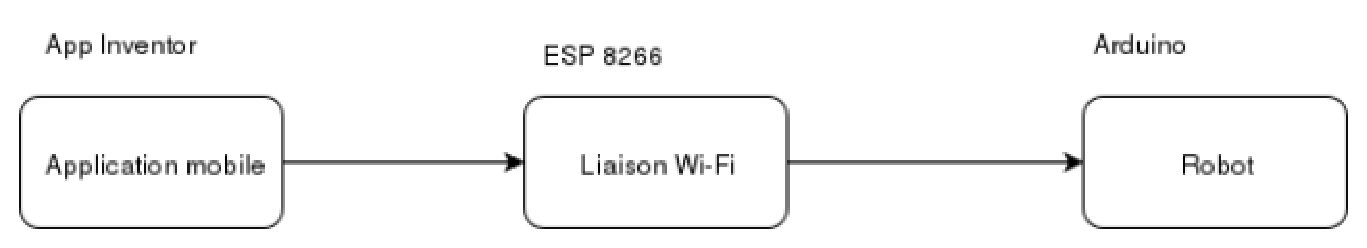
\includegraphics[width=\linewidth]{SchemaBloc-svg.eps}
    \end{frame}


\section{Travail effectué}

    \begin{frame}{\insertsection}{Cahier de charges}
        \begin{itemize}
            \item Application mobile :
                \begin{itemize}
                    \item Interface graphique (photo)
                    \item Accéléromètre
                \end{itemize}
            \item Module Wi-Fi :
                \begin{description}
                    \item[ESP :] Serveur 
                    \item[Téléphone : ] Client
                \end{description}
            \item Robot
                \begin{itemize}
                    \item Programme Arduino : Exploitation des données reçues et transcriptionn en signal pour le moteur 
                \end{itemize}
        \end{itemize}
    \end{frame}


    \begin{frame}{\insertsection}{Module Wi-Fi ESP 8266}
        \begin{itemize}
            \item Communication série : Ordinateur / ESP8266 : \textcolor{blue}{MANUEL}
            
                 $\rightarrow $ Commandes  AT
                
        \end{itemize}
        
        \begin{itemize}
             \item Programme d'initialisation :  \textcolor{blue}{AUTOMATIQUE}
             
                 $\rightarrow $ fonction  \textit{SendCommande()}
                
        \end{itemize}
        
    \end{frame}
    
    \begin{frame}{\insertsection}{Application téléphone}
        \begin{description}
            \item[Envrionnement de développement : ] App inventor
            \item[Plateforme de sortie : ] Téléphone Android
            \item[Signaux d'entrée de sortie : ] Accéléromètre et Trames
        \end{description}
    \end{frame}

\section{Planification du travail restant}

    \begin{frame}{\insertsection}
    
    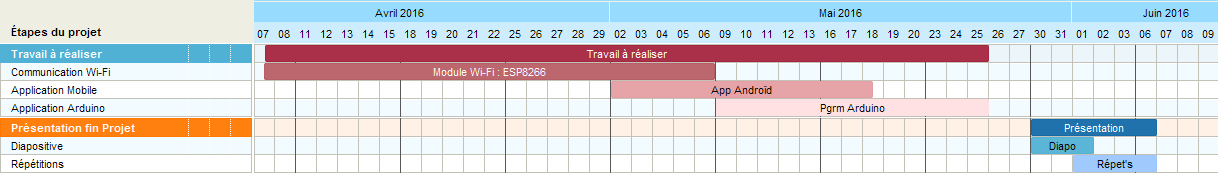
\includegraphics[width=\linewidth]{planning}
    
        Travail encadré (4 séances restantes) :
        \begin{itemize}
            \item Module Wi-Fi
        \end{itemize}
        
        Travail non encadré : 
        \begin{itemize}
            \item Hugo : Programme Arduino
            \item Claude-Alban : Programme Android
        \end{itemize}
    
    \end{frame}

\section{Annexes}

    \begin{frame}{\insertsection}
      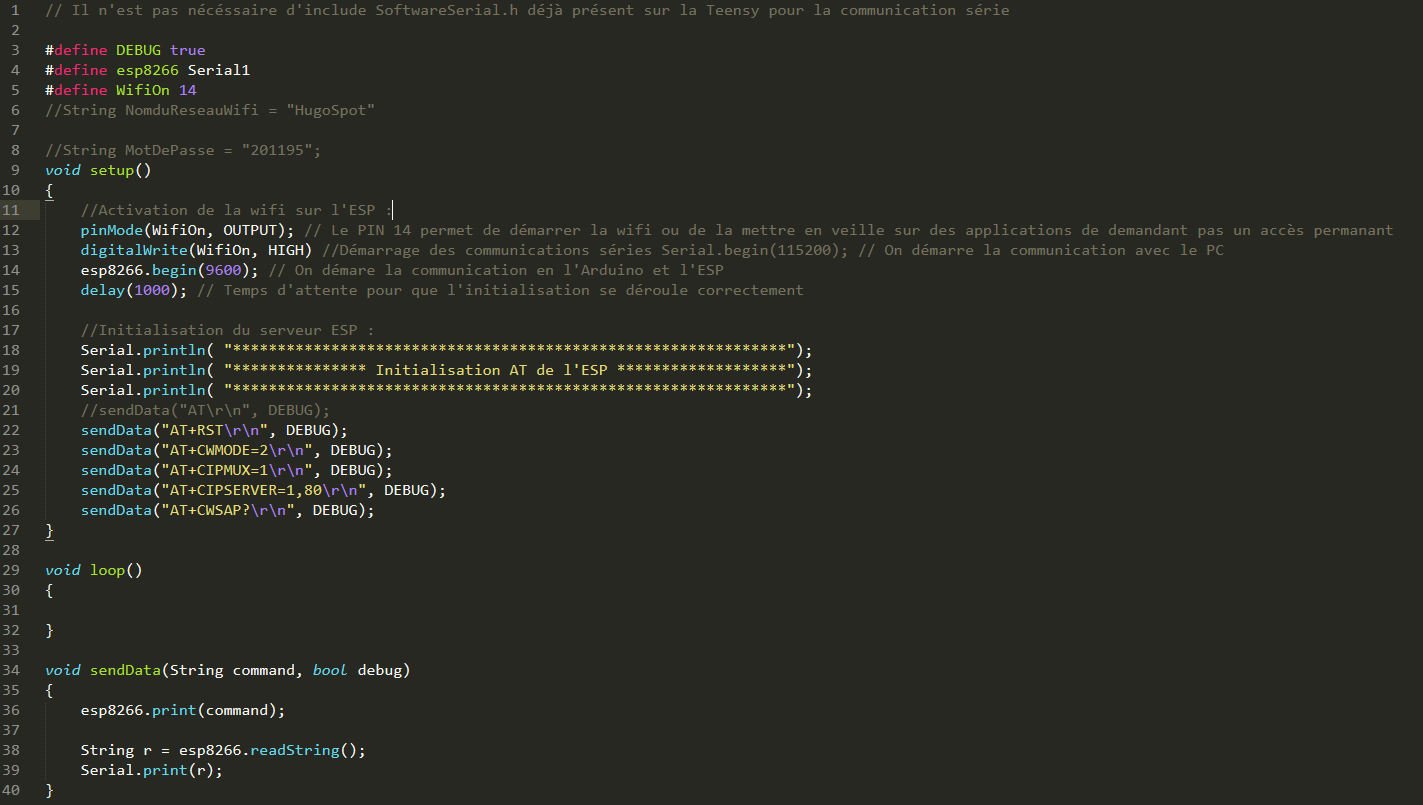
\includegraphics[width=\linewidth]{CodeESP}
    \end{frame}

\end{document}

